% vim: foldmethod=marker foldmarker=(fold),(end)
\documentclass{article}

% Setup (fold)
\usepackage[a4paper, margin=20mm]{geometry}
\usepackage{amsmath}
\usepackage{amsthm}
\usepackage{amssymb}
\usepackage{graphicx}
\usepackage{enumitem}
\usepackage{listings}
\usepackage{xcolor}

% Define code listing style
\lstdefinestyle{mystyle}{
	basicstyle=\ttfamily,
	keywordstyle=\color{blue},
	commentstyle=\color{green!60!black},
	stringstyle=\color{red},
	frame=single,
	breaklines=true,
	postbreak=\mbox{\textcolor{red}{$\hookrightarrow$}\space},
}

\lstset{style=mystyle}
\geometry{letterpaper, margin=1in}
\def\c#1{\texttt{#1}}

\title{Homework 4 - Information Security (ICS344)}
\author{Alfaifi, Ammar -- 201855360}
\date{\today}
% Setup (end)

\begin{document}
\maketitle

\section{Firewalls and Connection Tracking} % (fold)
\label{sec:Firewalls and Connection Tracking}
My machine is iMac M1, and I don't have easy access to Virtualbox capabilties, so I'll use three real machines for this setup.
\begin{enumerate}
	\item iMac with macOS as Node A.
	\item Labtop with Arch Linux as Router.
	\item Raspberry Pi as Node B.
\end{enumerate}

Now to setup Arch Linux as router I follow theses steps:
\begin{enumerate}
	\item Assign the IP address \c{192.168.60.11} to the network interface card (NIC) named \c{enp7s0u1u2i5}
	      and optionally enable a DHCP server to assign an IP address when a new device connects. This is by adding
	      the following configs to file \c{/etc/systemda/network/20-dhcpd-wired.network}:
	      \begin{lstlisting}[language=bash, caption={Assign IP addresses to interfaces}]
[Match]
Name=enp7s0u1u2i5

[Network]
Address=192.168.60.11/24
DHCPServer=true
IPMasquerade=ipv4


[DHCPServer]
PoolOffset=100
PoolSize=20
EmitDNS=yes
DNS=9.9.9.9
\end{lstlisting}
	      \begin{itemize}
		      \item \textbf{DHCPServer} Enables the DHCP server on the specified network interface. This means the machine will be providing dynamic IP addresses to other devices on the network.
		      \item \textbf{IPMasquerade} Configures IP masquerading for IPv4. This is typically used in network address translation (NAT) cenarios, allowing devices with private IP addresses to access the internet using the public IP address of the machine running the masquerading.
	      \end{itemize}
	\item Doing the same for other NIC, but only change \c{Address} config to \c{10.1.1.0/24},
	      and \c{Name=wlp2s0}. And write it
	      to another file in folder \c{/etc/systemd/network/}

	\item to allow Arch OS to forward packets as needed we enable that by, running the following:
	      \begin{lstlisting}[language=bash, caption={Enable port forwarding}]
  sudo sysctl net.ipv4.ip_forward=1
  sudo sysctl net.ipv4.conf.all.forwarding=1
  sudo sysctl net.ipv6.conf.all.forwarding=1
    \end{lstlisting}
	\item Lastly we reload configs by running \c{sudo networkctl reload}.
\end{enumerate}

\subsection{Results} % (fold)
\label{sub:Results}
\begin{itemize}
	\item See Figure~\ref{fig:interfaces} for the Router interfaces settings after settuing up
	      the configs above.
	\item See Figure~\ref{fig:ping-router}, when Router is being ping from Node A.
	\item See Figure~\ref{fig:ping-node-b}, when Node B is being ping from Node A, and Figure~\ref{fig:ping-node-b-wire} for
	      wireshark logs.
	\item See Figure~\ref{fig:not-reach} where after configuring Router not to forward packets
	      from Node B to Node A.
\end{itemize}

\begin{figure}[!hb]
	\centering
	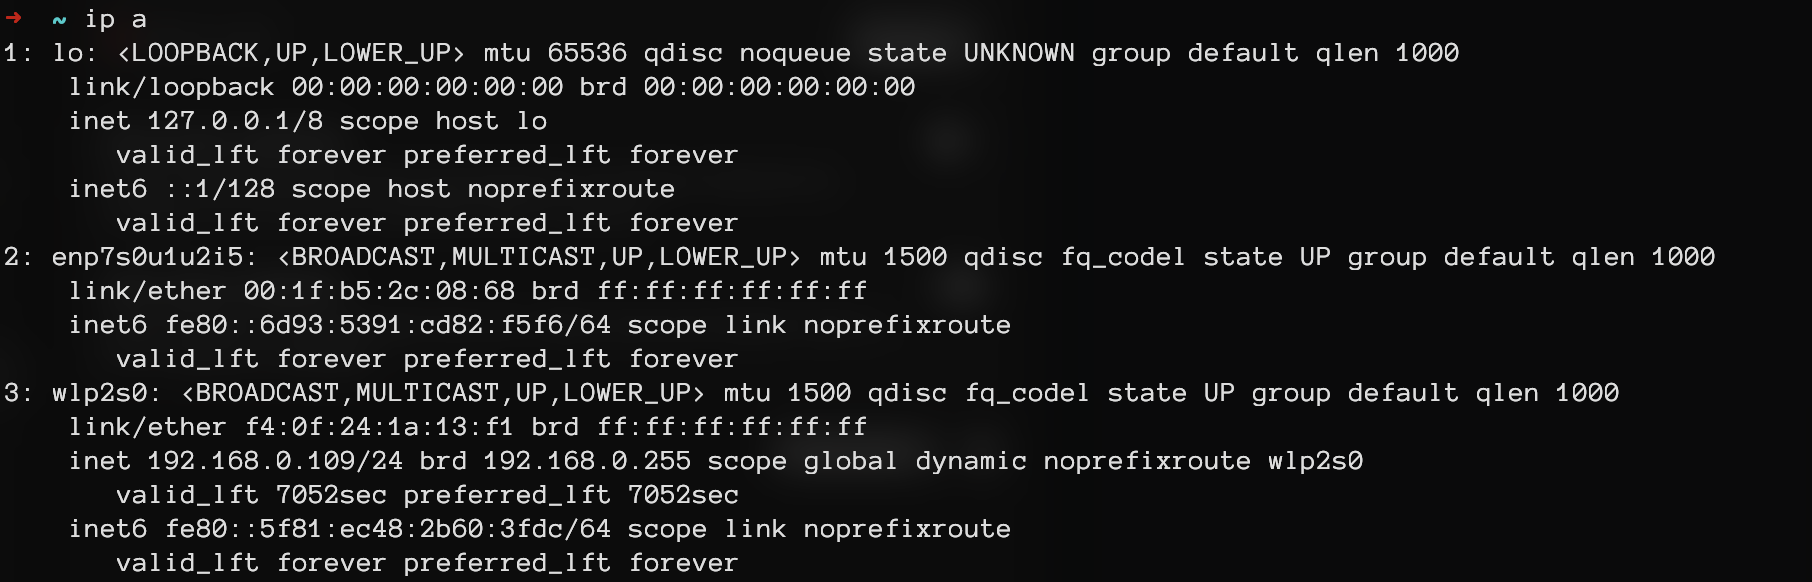
\includegraphics[width=0.8\textwidth]{figures/interfaces}
	\caption{IP and MAC addresses for the of the Router}
	\label{fig:interfaces}
\end{figure}

\begin{figure}[!hb]
	\centering
	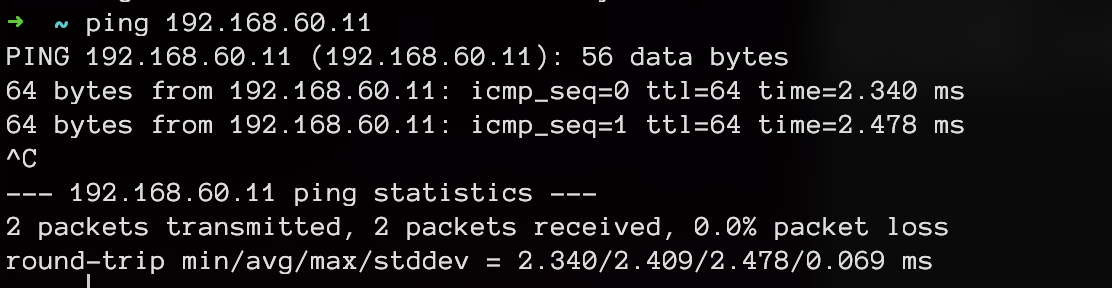
\includegraphics[width=0.8\textwidth]{figures/ping-router}
	\caption{Router is ping-ed from Node A}
	\label{fig:ping-router}
\end{figure}

\begin{figure}[!hb]
	\centering
	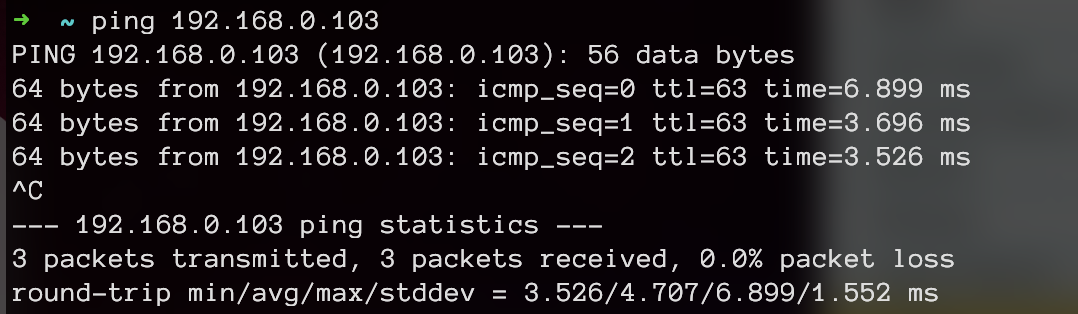
\includegraphics[width=0.8\textwidth]{figures/ping-node-b}
	\caption{Ping Node B from Node A.}
	\label{fig:ping-node-b}
\end{figure}

\begin{figure}[!hb]
	\centering
	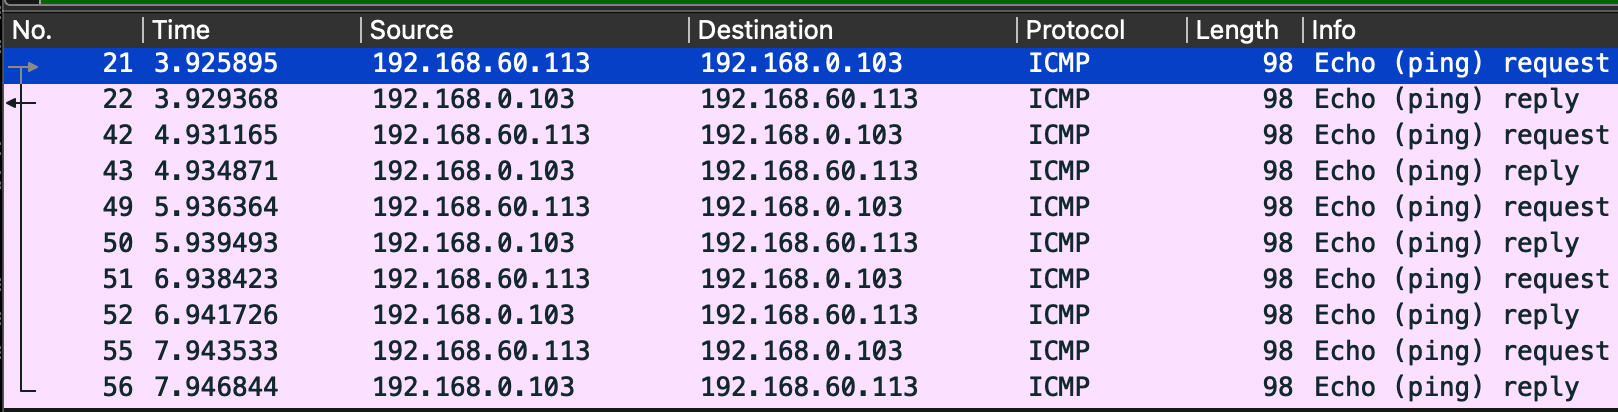
\includegraphics[width=0.8\textwidth]{figures/ping-b-wire}
	\caption{Wireshark catching ICMP packets when ping Node B from Node A.}
	\label{fig:ping-node-b-wire}
\end{figure}

\begin{figure}[!hb]
	\centering
	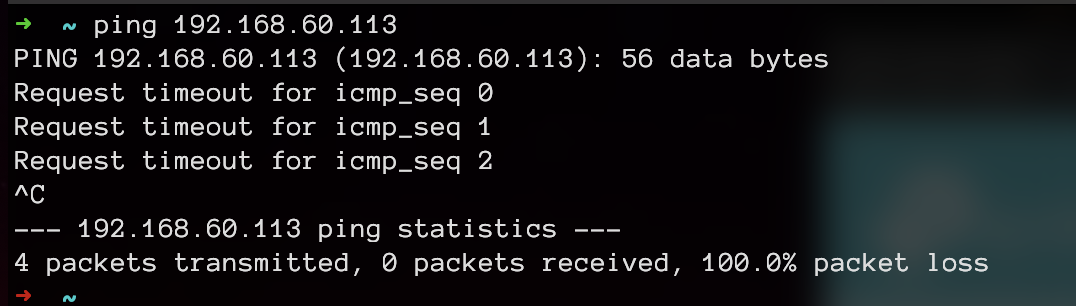
\includegraphics[width=0.8\textwidth]{figures/not-reach}
	\caption{Node A is not reachable from Node B.}
	\label{fig:not-reach}
\end{figure}
% subsection Results (end)
% section Firewalls and Connection Tracking (end)

\section{TUN Interface} % (fold)
\label{sec:TUN Interface}
See Figure~\ref{fig:create-tun} for how to create TUN in Router as well as the
all the links active on Router including my TUN. In Figure~\ref{fig:assign-addr} I assigned
the IP address \c{192.168.60.60/24} to my TUN. Finaly Figure~\ref{fig:ping-tun} shows
\c{alfaifi-tun0} with IP address \c{192.168.60.60} is reachable from Node A.

\begin{figure}[!hb]
	\centering
	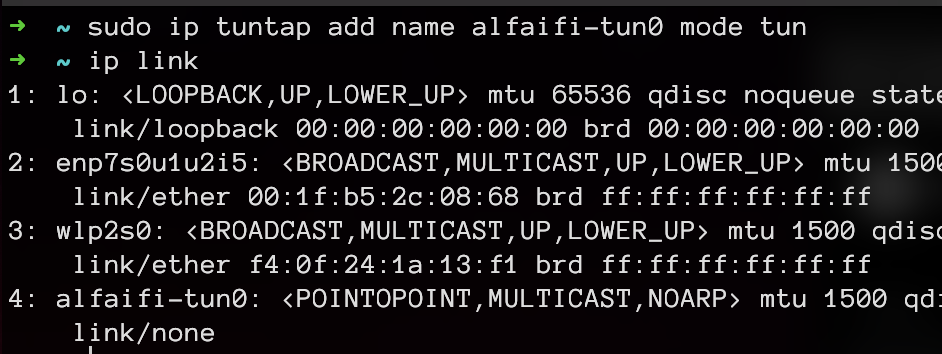
\includegraphics[width=0.8\textwidth]{./figures/create-tun.png}
	\caption{Shows command to create a TUN and the shows the all links on Router.}
	\label{fig:create-tun}
\end{figure}

\begin{figure}[!hb]
	\centering
	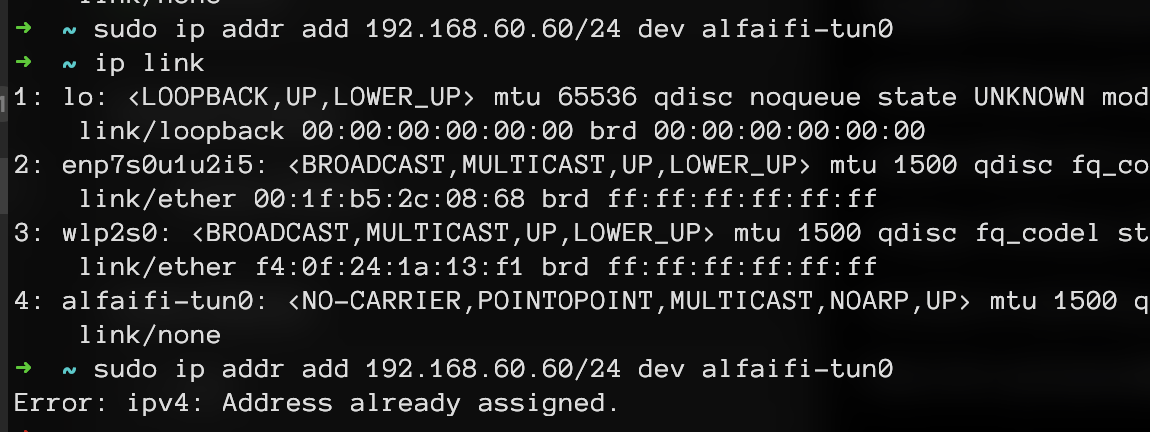
\includegraphics[width=0.8\textwidth]{./figures/assign-addr.png}
	\caption{Assign an IP address to my TUN.}
	\label{fig:assign-addr}
\end{figure}

\begin{figure}[!hb]
	\centering
	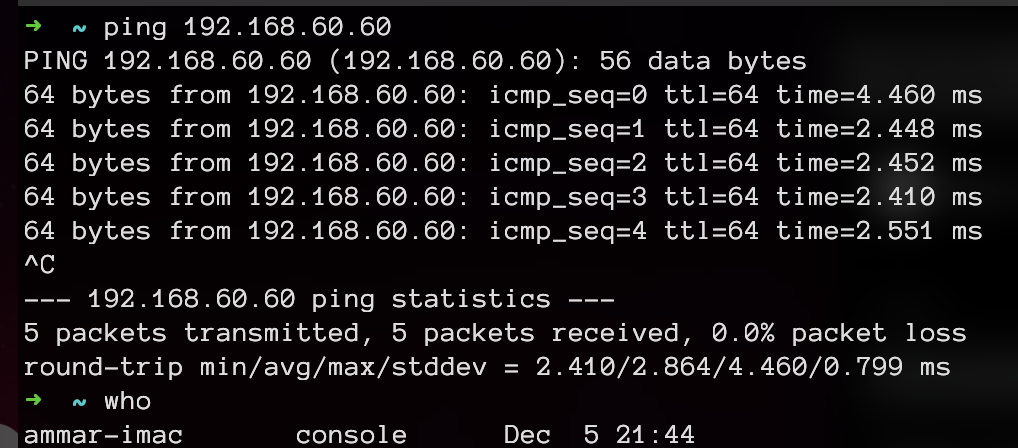
\includegraphics[width=0.8\textwidth]{./figures/ping-tun.png}
	\caption{Ping my TUN named \c{alfaifi-tun} from Node A.}
	\label{fig:ping-tun}
\end{figure}
% section TUN Interface (end)

\section{SQL Injection Attack} % (fold)
\label{sec:SQL Injection Attack}
In Figure~\ref{fig:create-table}, I created the table in a PosgreSQL database. And in Figure~\ref{fig:populate}
I populated it with some fake data.

Heres the code to create a simple python server to execute SQL query that has
threat of SQL injection attack:

\begin{lstlisting}[language=python, caption={Login server connected to DB}]
from flask import Flask, render_template, request
import psycopg2

app = Flask(__name__)

# PostgreSQL database configuration
db_config = {
    "dbname": "postgres",
    "user": "ammar-imac",
    "password": "",
    "host": "localhost",
    "port": "5432",
}


def execute_query(query, fetchall=True):
    try:
        connection = psycopg2.connect(**db_config)
        cursor = connection.cursor()
        cursor.execute(query)
        result = cursor.fetchall() if fetchall else cursor.fetchone()
        connection.commit()
        cursor.close()
        connection.close()

        return result
    except Exception as e:
        return str(e)


@app.route("/")
def index():
    return render_template("login.html")


@app.route("/login", methods=["POST"])
def login():
    username = request.form.get("username")
    password = request.form.get("password")

    if not username or not password:
        return render_template(
            "login.html", error="Username and password are required."
        )

    query = (
        f"SELECT * FROM Employee WHERE Email='{username}' AND Password='{password}';"
    )
    result = execute_query(query, fetchall=False)

    print(result)
    if result:
        return f"Welcome, {username}!"
    else:
        return render_template(
            "login.html", error="Invalid credentials. Please try again."
        )


if __name__ == "__main__":
    app.run(debug=True)
\end{lstlisting}


\subsection{Performing Attack} % (fold)
\label{sub:Performing Attack}
Figure~\ref{fig:login} shows an example of successull login.
Now to trick DB to return the entire table we'll use the fact \c{OR ''=''} is always TRUE.
See Figure~\ref{fig:injection}, how we enter this trick in username input and password.
Then from our code the server will substitute this values as a string into the SQL query.
It'll be like this before execute:
\begin{lstlisting}
SELECT * FROM Employee WHERE Email='' or ''='' AND Password='' or ''='';
\end{lstlisting}
Meaning every row in the table is returned and the attack is carried on, as seen
in Figure~\ref{fig:attacked} the returned employees' names and password.
% subsection Performing Attack (end)
\paragraph*{} Now I can use one of employees breached data to login and the result as in Figure~\ref{fig:login}.


\begin{figure}[hb]
	\centering
	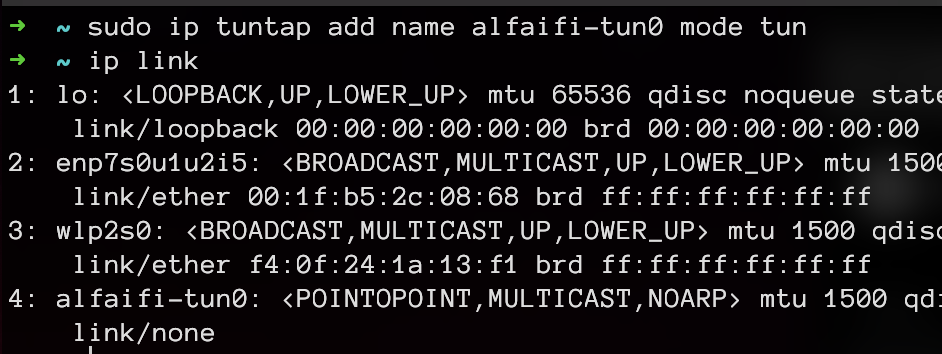
\includegraphics[width=0.8\textwidth]{./figures/create-tun.png}
	\caption{Create table \c{Empolyee}.}
	\label{fig:create-table}
\end{figure}

\begin{figure}[hb]
	\centering
	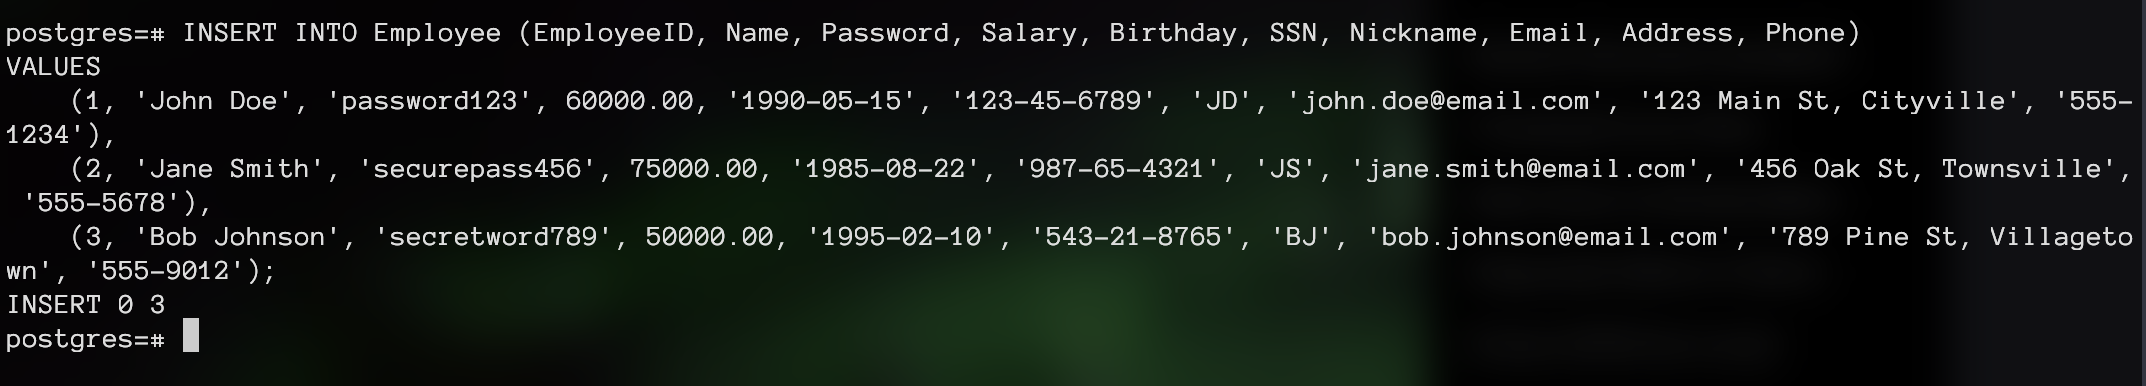
\includegraphics[width=0.8\textwidth]{./figures/populate.png}
	\caption{Populate table woith some data.}
	\label{fig:populate}
\end{figure}

\begin{figure}[hb]
	\centering
	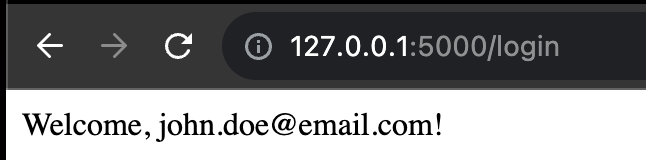
\includegraphics[width=0.8\textwidth]{./figures/login.png}
	\caption{A successull login with credentials matched from db.}
	\label{fig:login}
\end{figure}

\begin{figure}[hb]
	\centering
	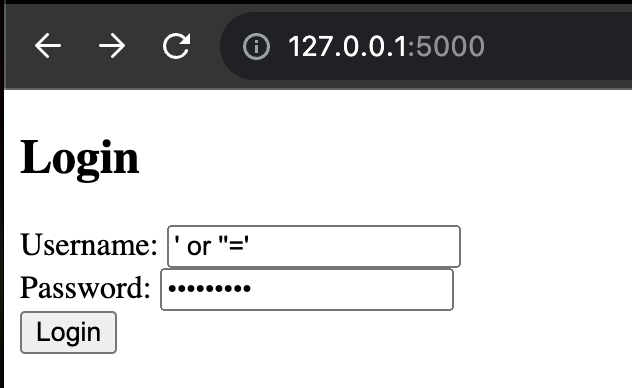
\includegraphics[width=0.8\textwidth]{./figures/sql-injection.png}
	\caption{Instead of real user data, here's we try to do an SQL injection}
	\label{fig:injection}
\end{figure}

\begin{figure}[hb]
	\centering
	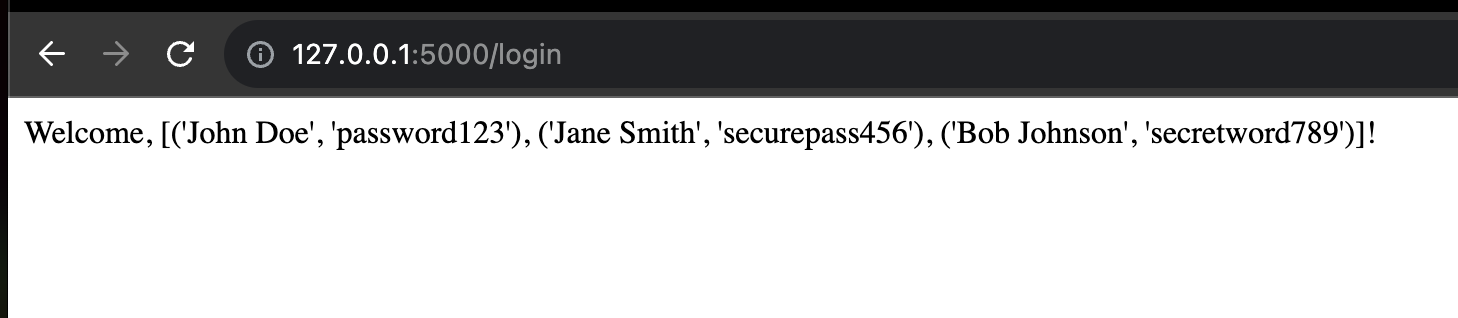
\includegraphics[width=0.8\textwidth]{./figures/attacked.png}
	\caption{After a successul attack, db returns matches the entire \c{Employee} table.}
	\label{fig:attacked}
\end{figure}
% section SQL Injection Attack (end)

\end{document}
